% =====================================================================
%  Example paper for the LaTeX course.
%  Build:  latexmk -pdf main.tex      (or upload this folder to Overleaf)
%  Uses only standard TeX Live packages, so no image files are needed:
%  the figure is drawn with TikZ.
% =====================================================================
\documentclass[11pt]{article}

% ---------- Layout (fine for a standalone doc; NEVER do this with a venue template) ----------
\usepackage[letterpaper, margin=1in]{geometry}

% ---------- Fonts & encoding ----------
\usepackage[T1]{fontenc}
\usepackage{lmodern}
\usepackage{microtype}

% ---------- Math ----------
\usepackage{amsmath, amssymb, amsthm, mathtools, bm}

% ---------- Figures, tables, algorithms ----------
\usepackage{graphicx}
\usepackage{subcaption}
\usepackage{booktabs}
\usepackage{multirow}
\usepackage{siunitx}
\usepackage[table]{xcolor}
\usepackage{tikz}
\usetikzlibrary{arrows.meta, positioning}
\usepackage{algorithm}
\usepackage{algpseudocode}
\usepackage{enumitem}
\usepackage{tcolorbox}
\usepackage[version=4]{mhchem}
\usepackage{pifont}

% ---------- Theorems (needs thmtools for restatable) ----------
\usepackage{thmtools, thm-restate}

% ---------- Bibliography ----------
\usepackage[numbers, sort&compress]{natbib}

% ---------- Links (load late) ----------
\usepackage{hyperref}
\hypersetup{colorlinks=true, linkcolor=blue!70!black, citecolor=blue!70!black, urlcolor=magenta!70!black}
\usepackage[capitalize, noabbrev]{cleveref}

% ---------- Your notation & helpers ----------
% ====================== macros.tex ======================
% Method name: change it here and it changes everywhere.
\usepackage{xspace}
\newcommand{\method}{\textsc{TinyNet}\xspace}

% Number sets, probability, losses
\newcommand{\R}{\mathbb{R}}
\newcommand{\E}{\mathbb{E}}
\newcommand{\D}{\mathcal{D}}
\newcommand{\loss}{\mathcal{L}}

% Vectors / matrices
\newcommand{\vx}{\bm{x}}
\newcommand{\vy}{\bm{y}}
\newcommand{\vz}{\bm{z}}
\newcommand{\vtheta}{\bm{\theta}}
\newcommand{\mW}{\mathbf{W}}
\newcommand{\tran}{^{\top}}

% Delimiters & operators
\DeclarePairedDelimiter{\norm}{\lVert}{\rVert}
\DeclarePairedDelimiter{\abs}{\lvert}{\rvert}
\DeclareMathOperator*{\argmin}{arg\,min}
\DeclareMathOperator*{\argmax}{arg\,max}
\DeclareMathOperator{\softmax}{softmax}

% Theorem environments
\theoremstyle{plain}
\newtheorem{theorem}{Theorem}[section]
\newtheorem{lemma}[theorem]{Lemma}
\theoremstyle{definition}
\newtheorem{assumption}{Assumption}
\newtheorem{definition}[theorem]{Definition}
\crefname{assumption}{Assumption}{Assumptions}

% Table helpers
\newcommand{\cmark}{\ding{51}}
\newcommand{\xmark}{\ding{55}}
\newcommand{\pmstd}[1]{{\scriptsize$\pm$#1}}

% Collaboration notes; comment out the second line block to hide them
\newcommand{\todo}[1]{\textcolor{red}{[TODO: #1]}}
\newcommand{\ada}[1]{\textcolor{blue}{[Ada: #1]}}
% \renewcommand{\todo}[1]{}
% \renewcommand{\ada}[1]{}


% ---------------------------------------------------------------------
\title{\method: A Tiny Example Paper\\for Learning \LaTeX{}}
\author{
  Ada Lovelace\thanks{Equal contribution.} \\
  Analytical Engine Lab\\
  \texttt{ada@example.org}
  \and
  Alan Turing\footnotemark[1] \\
  Bletchley Institute\\
  \texttt{alan@example.org}
}
\date{}

\begin{document}
\maketitle

\begin{abstract}
  We present \method, a deliberately simple method whose only purpose is to
  show how common elements of a machine learning paper are written in \LaTeX{}:
  equations, theorems, figures, tables, algorithms and citations.
  On a made-up benchmark, \method improves accuracy by \qty{1.1}{\percent}
  while using \num{40e6} parameters.
\end{abstract}

\section{Introduction}\label{sec:intro}
% Tip: one sentence per line makes git diffs readable.
Deep networks are trained by minimizing an empirical risk~\citep{goodfellow2016deep}.
\citet{vaswani2017attention} introduced the Transformer, which is now everywhere~\citep{lecun2015deep, vaswani2017attention}.
In this paper we propose \method, shown in \cref{fig:arch}.

\begin{figure}[t]
  \centering
  % TikZ figure, included with % TikZ figure, included with \input{figures/architecture}
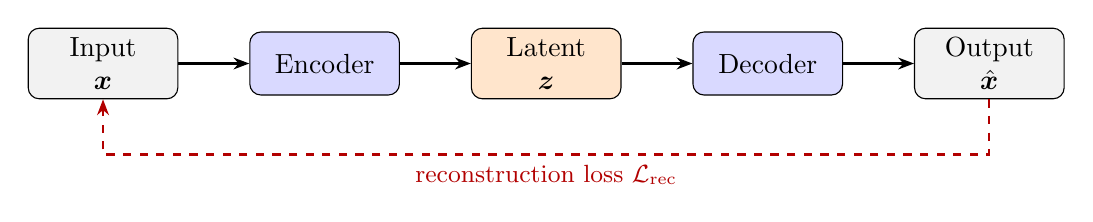
\begin{tikzpicture}[
    node distance=0.9cm,
    box/.style={draw, rounded corners, minimum width=1.9cm, minimum height=0.8cm,
                align=center, fill=#1},
    box/.default=white,
    arrow/.style={-{Stealth[length=2mm]}, thick},
  ]
  \node[box=gray!10]                 (input) {Input\\$\vx$};
  \node[box=blue!15, right=of input] (enc)   {Encoder};
  \node[box=orange!20, right=of enc] (lat)   {Latent\\$\vz$};
  \node[box=blue!15, right=of lat]   (dec)   {Decoder};
  \node[box=gray!10, right=of dec]   (out)   {Output\\$\hat{\vx}$};

  \draw[arrow] (input) -- (enc);
  \draw[arrow] (enc)   -- (lat);
  \draw[arrow] (lat)   -- (dec);
  \draw[arrow] (dec)   -- (out);
  \draw[arrow, dashed, red!70!black] (out.south) -- ++(0,-0.7)
      -| node[pos=0.25, below] {\small reconstruction loss $\loss_{\text{rec}}$} (input.south);
\end{tikzpicture}

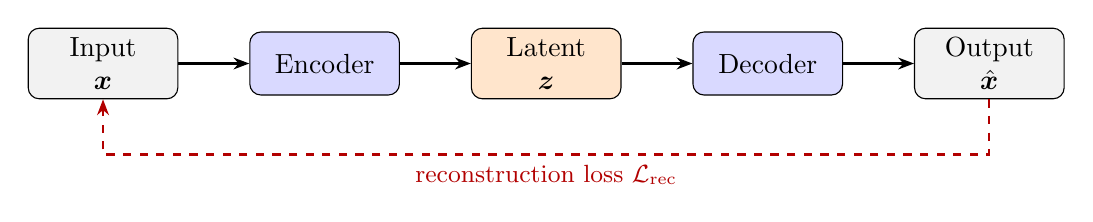
\begin{tikzpicture}[
    node distance=0.9cm,
    box/.style={draw, rounded corners, minimum width=1.9cm, minimum height=0.8cm,
                align=center, fill=#1},
    box/.default=white,
    arrow/.style={-{Stealth[length=2mm]}, thick},
  ]
  \node[box=gray!10]                 (input) {Input\\$\vx$};
  \node[box=blue!15, right=of input] (enc)   {Encoder};
  \node[box=orange!20, right=of enc] (lat)   {Latent\\$\vz$};
  \node[box=blue!15, right=of lat]   (dec)   {Decoder};
  \node[box=gray!10, right=of dec]   (out)   {Output\\$\hat{\vx}$};

  \draw[arrow] (input) -- (enc);
  \draw[arrow] (enc)   -- (lat);
  \draw[arrow] (lat)   -- (dec);
  \draw[arrow] (dec)   -- (out);
  \draw[arrow, dashed, red!70!black] (out.south) -- ++(0,-0.7)
      -| node[pos=0.25, below] {\small reconstruction loss $\loss_{\text{rec}}$} (input.south);
\end{tikzpicture}

  \caption{\textbf{Overview of \method.} An encoder maps the input $\vx$ to a latent $\vz$,
    and a decoder reconstructs $\hat{\vx}$. The dashed arrow is the reconstruction loss.}
  \label{fig:arch}
\end{figure}

\paragraph{Contributions.} Our main contributions are:
\begin{itemize}[leftmargin=*, nosep]
  \item a simple objective (\cref{sec:method}, \cref{eq:objective});
  \item a convergence guarantee (\cref{thm:conv});
  \item experiments showing gains on two benchmarks (\cref{tab:main}).
\end{itemize}

\begin{tcolorbox}[colback=blue!4, colframe=blue!50!black, title=Key idea]
  Reconstruct first, then classify. Everything else is detail.
\end{tcolorbox}

Even chemistry fits: combustion of methane is \ce{CH4 + 2O2 -> CO2 + 2H2O}.
\ada{Do we really need the chemistry sentence?}

\section{Method}\label{sec:method}

\paragraph{Setup.}
Let $\D = \{(\vx_i, y_i)\}_{i=1}^{n}$ with $\vx_i \in \R^d$ and $y_i \in \{1, \ldots, K\}$.
A model $f_{\vtheta} \colon \R^d \to \R^K$ produces logits $\vz = f_{\vtheta}(\vx)$.

% ---- Exercise 1 from Chapter 4: softmax ----
The predicted class probabilities are given by the softmax
\begin{equation}
  \sigma(\vz)_i = \frac{\exp(z_i)}{\sum_{j=1}^{K} \exp(z_j)}, \qquad i = 1, \ldots, K.
  \label{eq:softmax}
\end{equation}

% ---- Exercise 2: attention with \softmax as an operator ----
Our encoder uses scaled dot-product attention~\citep{vaswani2017attention},
\[
  \mathrm{Attn}(Q, K, V) = \softmax\!\left( \frac{Q K\tran}{\sqrt{d_k}} \right) V .
\]

\paragraph{Objective.}
We minimize cross-entropy plus a reconstruction term weighted by $\lambda \ge 0$:
\begin{equation}
  \vtheta^\star = \argmin_{\vtheta} \;
  \underbrace{-\frac{1}{n}\sum_{i=1}^{n} \log \sigma\bigl(f_{\vtheta}(\vx_i)\bigr)_{y_i}}_{\loss_{\text{CE}}}
  + \lambda \, \loss_{\text{rec}}(\vtheta).
  \label{eq:objective}
\end{equation}

% ---- Exercise 3: align, only the last line numbered ----
For intuition, for a linear model with squared error,
\begin{align}
  \nabla_{\vtheta} \frac{1}{2n}\norm{\mW\vtheta - \vy}^2
    &= \frac{1}{2n} \nabla_{\vtheta} (\mW\vtheta - \vy)\tran(\mW\vtheta - \vy) \nonumber \\
    &= \frac{1}{2n} \cdot 2\, \mW\tran (\mW\vtheta - \vy) \nonumber \\
    &= \frac{1}{n} \mW\tran (\mW\vtheta - \vy). \label{eq:mse-grad}
\end{align}

A piecewise activation, for completeness:
\[
  \mathrm{ReLU}(x) =
  \begin{cases}
    x & \text{if } x > 0, \\
    0 & \text{otherwise.}
  \end{cases}
\]

\paragraph{Optimization.} We train with SGD (\cref{alg:sgd}).

\begin{algorithm}[t]
  \caption{Training \method with mini-batch SGD}
  \label{alg:sgd}
  \begin{algorithmic}[1]
    \Require dataset $\D$, learning rate $\eta$, epochs $T$, weight $\lambda$
    \Ensure parameters $\vtheta$
    \State initialize $\vtheta_0$
    \For{$t = 1$ \textbf{to} $T$}
      \For{each minibatch $B \subset \D$}
        \State $g \gets \nabla_{\vtheta} \bigl[\loss_{\text{CE}}(B) + \lambda \loss_{\text{rec}}(B)\bigr]$
        \State $\vtheta \gets \vtheta - \eta\, g$ \Comment{gradient step}
      \EndFor
    \EndFor
    \State \Return $\vtheta$
  \end{algorithmic}
\end{algorithm}

\paragraph{Theory.}

\begin{assumption}[Smoothness]\label{asm:smooth}
  The objective $\loss$ is $\beta$-smooth and bounded below by $\loss^\star$.
\end{assumption}

% ---- Exercise 4: restatable theorem; proof (with \qedhere) is in the appendix ----
\begin{restatable}[Convergence]{theorem}{convthm}\label{thm:conv}
  Under \cref{asm:smooth}, gradient descent with step size $\eta \le 1/\beta$ satisfies
  \[
    \min_{t < T} \norm{\nabla \loss(\vtheta_t)}^2 \le \frac{2\bigl(\loss(\vtheta_0) - \loss^\star\bigr)}{\eta T}.
  \]
\end{restatable}

The proof is in \cref{app:proofs}.

\section{Experiments}\label{sec:experiments}

\paragraph{Datasets.} We use two made-up benchmarks, \textsc{Toy-10} and \textsc{Toy-1k}.

\paragraph{Hardware.} Training takes \qty{3.5}{\hour} on one GPU with \qty{80}{\giga\byte} of memory.

\paragraph{Results.} \Cref{tab:main} shows the main results.
\method is best on both benchmarks, and \cref{tab:features} compares capabilities.
\todo{add error bars from 5 seeds}

\begin{table}[t]
  \centering
  \caption{Accuracy (\%) on two benchmarks, mean \pmstd{std} over 3 seeds.
    Best in \textbf{bold}, second best \underline{underlined}.}
  \label{tab:main}
  \small
  \begin{tabular}{@{}lcccc@{}}
    \toprule
    \multirow{2}{*}{Method} & \multicolumn{2}{c}{\textsc{Toy-10}} & \multicolumn{2}{c}{\textsc{Toy-1k}} \\
    \cmidrule(lr){2-3} \cmidrule(lr){4-5}
                     & Top-1 & Params & Top-1 & Params \\
    \midrule
    MLP              & 88.2\pmstd{0.4}             & 5M  & 61.3\pmstd{0.6}             & 5M  \\
    Transformer      & \underline{91.0}\pmstd{0.3} & 86M & \underline{70.4}\pmstd{0.5} & 86M \\
    \rowcolor{blue!6}
    \method (ours)   & \textbf{92.1}\pmstd{0.2}    & 40M & \textbf{71.5}\pmstd{0.4}    & 40M \\
    \bottomrule
  \end{tabular}
\end{table}

\begin{table}[t]
  \centering
  \caption{Feature comparison.}
  \label{tab:features}
  \small
  \begin{tabular}{@{}lccc@{}}
    \toprule
    Method      & Reconstruction & Attention & Guarantee \\
    \midrule
    MLP         & \xmark & \xmark & \xmark \\
    Transformer & \xmark & \cmark & \xmark \\
    \method     & \cmark & \cmark & \cmark \\
    \bottomrule
  \end{tabular}
\end{table}

\begin{figure}[t]
  \centering
  \begin{subfigure}[b]{0.48\linewidth}
    \centering
    % In a real paper: \includegraphics[width=\linewidth]{loss_curve}
    \fbox{\parbox[c][2.5cm][c]{0.9\linewidth}{\centering placeholder for\\ \texttt{loss\_curve.pdf}}}
    \caption{Training loss.}
    \label{fig:loss}
  \end{subfigure}
  \hfill
  \begin{subfigure}[b]{0.48\linewidth}
    \centering
    \fbox{\parbox[c][2.5cm][c]{0.9\linewidth}{\centering placeholder for\\ \texttt{accuracy.pdf}}}
    \caption{Test accuracy.}
    \label{fig:acc}
  \end{subfigure}
  \caption{Training dynamics. \Cref{fig:loss} shows the loss and \cref{fig:acc} the accuracy.}
  \label{fig:dynamics}
\end{figure}

\Cref{fig:dynamics} shows training curves.


\section{Conclusion}\label{sec:conclusion}
We showed how to write a paper in \LaTeX{}. Limitations and the full proof are
in \cref{app:proofs}.

\section*{Acknowledgments}
We thank the readers of this course.

\bibliographystyle{plainnat}
\bibliography{refs}

\clearpage
\appendix
\section{Proofs}\label{app:proofs}

We restate \cref{thm:conv} for convenience. It keeps its original number.

\convthm*

\begin{proof}
  By $\beta$-smoothness and $\eta \le 1/\beta$, each step decreases the objective:
  $\loss(\vtheta_{t+1}) \le \loss(\vtheta_t) - \frac{\eta}{2}\norm{\nabla\loss(\vtheta_t)}^2$.
  Summing over $t = 0, \ldots, T-1$ and using $\loss(\vtheta_T) \ge \loss^\star$,
  \[
    T \min_{t<T} \norm{\nabla\loss(\vtheta_t)}^2
    \le \sum_{t=0}^{T-1} \norm{\nabla\loss(\vtheta_t)}^2
    \le \frac{2\bigl(\loss(\vtheta_0) - \loss^\star\bigr)}{\eta}. \qedhere
  \]
\end{proof}

\section{Hyperparameters}\label{app:hparams}

\begin{table}[h]
  \centering
  \caption{Hyperparameters.}
  \label{tab:hparams}
  \begin{tabular}{@{}ll@{}}
    \toprule
    Parameter & Value \\
    \midrule
    Learning rate $\eta$ & \num{3e-4} \\
    Weight decay         & \num{1e-2} \\
    Batch size           & \num{256} \\
    \bottomrule
  \end{tabular}
\end{table}


\end{document}
